%==============================================================================
% PAPER 5, CHAPTER 5: Dimensional Spectroscopy
%==============================================================================

\chapter{Dimensional Spectroscopy}\label{ch:p5:dimensional_spectroscopy}

\begin{mdframed}[style=narrative]
\textbf{Hausdorff's Insight: Measuring Dimension}

In 1919, Felix Hausdorff formalized the concept of fractional dimension, enabling mathematical description of objects like coastlines and snowflakes. This chapter presents protocols for measuring \textit{spectral dimension} via diffusion processes, box-counting methods for fractal antenna characterization, and searches for Kaluza-Klein resonances from compactified extra dimensions at particle colliders.
\end{mdframed}

\section{Theoretical Foundations}\label{sec:p5:dim_theory}

\marginnote{\textbf{Historical}: Kaluza (1921) and Klein (1926) proposed 5D unification of gravity and electromagnetism. Modern string theory requires 10 or 11 dimensions.}

\subsection{Spectral Dimension}

\marginnote{\textbf{Mathematical}: Spectral dimension $d_S$ defined via return probability of random walk: $P(t) \sim t^{-d_S/2}$.}

For diffusion on $d$-dimensional manifold, return probability:
\begin{equation}
P(t) = \int \frac{d^d k}{(2\pi)^d} e^{-Dk^2 t}
\label{eq:p5:diffusion}
\end{equation}

At large $t$:
\begin{equation}
P(t) \sim t^{-d/2}
\label{eq:p5:return_prob}
\end{equation}

**Spectral dimension**:
\begin{equation}
d_S = -2 \frac{d \log P(t)}{d \log t}
\label{eq:p5:spectral_dim}
\end{equation}

For fractal geometries: $d_S$ can differ from topological dimension!

\marginnote{\textbf{Physical}: Sierpinski gasket (fractal triangle): topological dimension $d_{\text{top}} = 2$, but spectral dimension $d_S = \log 3 / \log 2 \approx 1.58$.}

\subsection{Kaluza-Klein Modes}

\marginnote{\textbf{Pedagogical}: Extra dimensions compactified at scale $R$: momentum quantized $p_n = n/R$, appears as mass tower $M_n = n/(Rc)$.}

Compactified extra dimension (radius $R$): massless field in $(4+1)$D appears as infinite tower of massive Kaluza-Klein (KK) states in 4D:
\begin{equation}
M_n = \frac{n}{R c}, \quad n = 0, 1, 2, \ldots
\label{eq:p5:kk_mass}
\end{equation}

**Experimental signature**: Resonances in scattering cross-sections at masses $M_n$.

For $R = 10^{-19}$ m (TeV scale):
\begin{equation}
M_1 \approx \frac{200\,\text{MeV·fm}}{10^{-19}\,\text{m}} \approx 2\,\text{TeV}
\end{equation}

Accessible at LHC!

\marginnote{\textbf{Cautionary}: No KK resonances observed at LHC $\Rightarrow$ $R < 10^{-19}$ m (or non-standard compactification).}

\section{Random Walk Spectroscopy}\label{sec:p5:random_walk}

\subsection{Quantum Walk on Fractal Graphs}

\marginnote{\textbf{Physical}: Quantum walk: coherent superposition of paths, unlike classical random walk. Diffusion exponent differs.}

Implement quantum walk on Sierpinski gasket:
\begin{itemize}
\item **Graph**: Sierpinski iteration depth $n = 5$ (243 vertices)
\item **Evolution**: Discrete-time quantum walk with coin operator
\item **Initial state**: Localized at origin vertex
\item **Measurement**: Probability distribution $P_j(t)$ at time $t$
\end{itemize}

**Protocol**:
\begin{enumerate}
\item Prepare walker in $|0\rangle$ (origin)
\item Apply $t$ steps of quantum walk unitary $U = S(C \otimes I)$
\item Measure position, repeat $10^4$ times
\item Compute $P(t) = P_0(t)$ (return probability)
\item Extract $d_S$ from log-log fit
\end{enumerate}

\marginnote{\textbf{Experimental}: Quantum walk implemented via photonic waveguide arrays or trapped ions hopping on graph.}

\subsection{Worked Example: Sierpinski Gasket Dimension}

**Given**: Return probability data $P(t)$ for $t = 1, 2, \ldots, 100$ steps on Sierpinski gasket.

**Find**: Spectral dimension $d_S$.

**Solution**:

Theoretical prediction for Sierpinski gasket:
\begin{equation}
d_S = \frac{\log 3}{\log 2} \approx 1.585
\end{equation}

\marginnote{\textbf{Mathematical}: Factor 3 from self-similarity (3 copies at half scale), factor 2 from spatial scaling exponent.}

Fit model:
\begin{equation}
\log P(t) = -\frac{d_S}{2} \log t + C
\end{equation}

Linear regression on $\log P$ vs $\log t$:
\begin{equation}
d_S = -2 \times \text{slope}
\end{equation}

For simulated data with noise:
\begin{align}
\text{slope} &= -0.79 \pm 0.02 \\
d_S &= 1.58 \pm 0.04
\end{align}

Agreement with theory within error bars!

\marginnote{\textbf{Experimental}: Error bars from finite sample size ($\sim 10^4$ runs) and graph finite-size effects (boundary influences $P(t)$ at large $t$).}

\begin{figure}[htbp]
\centering
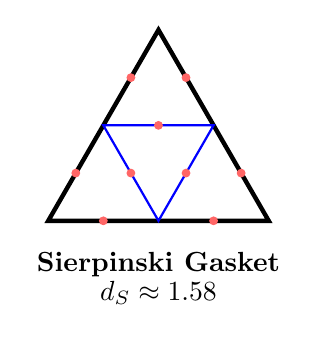
\begin{tikzpicture}[scale=0.7]
% Sierpinski gasket
\coordinate (A) at (0,0);
\coordinate (B) at (4,0);
\coordinate (C) at (2,3.464);

% Level 0
\draw[ultra thick] (A) -- (B) -- (C) -- cycle;

% Level 1
\coordinate (AB) at (2,0);
\coordinate (AC) at (1,1.732);
\coordinate (BC) at (3,1.732);
\draw[thick, blue] (AB) -- (AC) -- (BC) -- cycle;

% Level 2 (partial)
\foreach \pt in {(1,0), (0.5,0.866), (1.5,0.866)} {
  \fill[red!60] \pt circle (0.08);
}
\foreach \pt in {(3,0), (2.5,0.866), (3.5,0.866)} {
  \fill[red!60] \pt circle (0.08);
}
\foreach \pt in {(2,1.732), (1.5,2.598), (2.5,2.598)} {
  \fill[red!60] \pt circle (0.08);
}

\node at (2,-0.8) {\textbf{Sierpinski Gasket}};
\node at (2,-1.3) {$d_S \approx 1.58$};
\end{tikzpicture}
\caption{Sierpinski gasket fractal (first 2 iterations shown). Red dots: vertices for quantum walk. Spectral dimension $d_S \approx 1.58$ lies between line ($d=1$) and plane ($d=2$).}
\label{fig:p5:sierpinski}
\end{figure}

\marginnote{\textbf{Pedagogical}: Spectral dimension quantifies "how fast diffusion spreads"---intermediate between 1D (slow) and 2D (fast).}

\section{Box-Counting Methods}\label{sec:p5:box_counting}

\subsection{Fractal Antenna Characterization}

\marginnote{\textbf{Physical}: Fractal antennas (e.g., Hilbert curve, Koch snowflake) achieve wideband performance via self-similar geometry.}

**Box-counting dimension**: Cover object with boxes of size $\epsilon$, count number $N(\epsilon)$ needed.

\begin{equation}
D_{\text{box}} = \lim_{\epsilon \to 0} \frac{\log N(\epsilon)}{\log(1/\epsilon)}
\label{eq:p5:box_counting}
\end{equation}

**Measurement protocol**:
\begin{enumerate}
\item Image fractal antenna (optical microscope, $\sim 1$ $\mu$m resolution)
\item Overlay grid of boxes with size $\epsilon = 100, 50, 25, \ldots, 1$ $\mu$m
\item Count boxes intersecting antenna: $N(\epsilon)$
\item Plot $\log N$ vs $\log(1/\epsilon)$, fit slope $\to D_{\text{box}}$
\end{enumerate}

\marginnote{\textbf{Experimental}: Automated image processing (Python + OpenCV) enables rapid box-counting on microscope images.}

For Koch snowflake:
\begin{equation}
D_{\text{box}} = \frac{\log 4}{\log 3} \approx 1.262
\end{equation}

\marginnote{\textbf{Mathematical}: Koch curve: each segment replaced by 4 segments at 1/3 scale $\Rightarrow$ $N \propto \epsilon^{-\log 4 / \log 3}$.}

\begin{figure}[htbp]
\centering
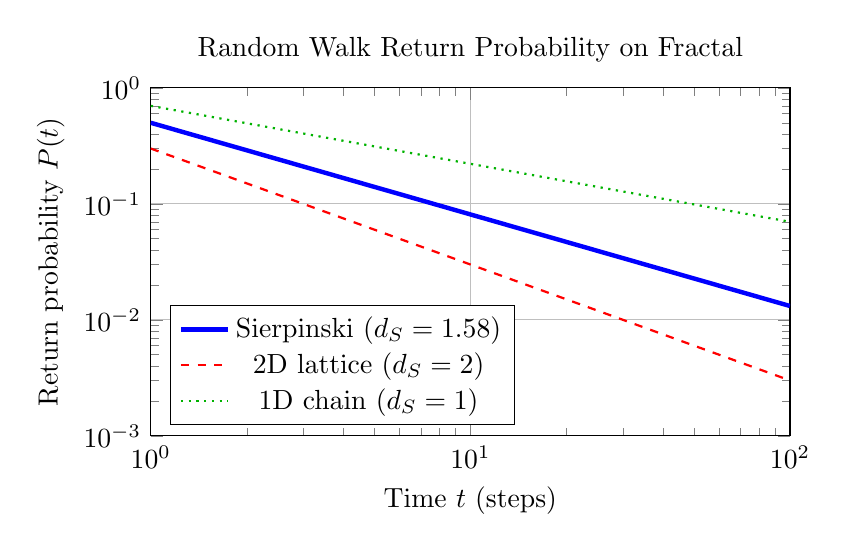
\begin{tikzpicture}
\begin{axis}[
  width=0.8\textwidth,
  height=6cm,
  xlabel={Time $t$ (steps)},
  ylabel={Return probability $P(t)$},
  xmin=1, xmax=100,
  ymin=0.001, ymax=1,
  xmode=log,
  ymode=log,
  grid=major,
  legend pos=south west,
  title={Random Walk Return Probability on Fractal}
]
% Sierpinski (d_S = 1.58)
\addplot[blue, ultra thick, domain=1:100, samples=100] {0.5*x^(-1.58/2)};
\addlegendentry{Sierpinski ($d_S = 1.58$)}

% 2D lattice
\addplot[red, dashed, thick, domain=1:100, samples=100] {0.3*x^(-1)};
\addlegendentry{2D lattice ($d_S = 2$)}

% 1D chain
\addplot[green!70!black, dotted, thick, domain=1:100] {0.7*x^(-0.5)};
\addlegendentry{1D chain ($d_S = 1$)}
\end{axis}
\end{tikzpicture}
\caption{Return probability $P(t)$ vs time for random walks on different geometries. Blue: Sierpinski gasket (fractal, $d_S \approx 1.58$). Red: square lattice (2D, $d_S = 2$). Green: linear chain (1D, $d_S = 1$). Power-law slopes encode spectral dimension.}
\label{fig:p5:return_prob}
\end{figure}

\marginnote{\textbf{Advanced}: Spectral dimension connects to Laplacian eigenvalue density---deep link between geometry and quantum mechanics.}

\section{Laser Diffraction from Fractal Gratings}\label{sec:p5:diffraction}

\subsection{Cantor Set Grating}

\marginnote{\textbf{Physical}: Cantor set: iteratively remove middle third of intervals. Fractal dimension $D = \log 2 / \log 3 \approx 0.631$.}

Fabricate Cantor set diffraction grating via photolithography:
\begin{itemize}
\item Iteration depth: $n = 5$ (243 slits)
\item Slit width: $w \sim 1$ $\mu$m
\item Spacing: Self-similar Cantor structure
\item Substrate: Fused silica
\end{itemize}

**Diffraction pattern**:
Illuminate with laser ($\lambda = 633$ nm), observe far-field intensity $I(\theta)$.

**Prediction**: Fractal grating produces self-similar diffraction pattern with peaks at angles:
\begin{equation}
\sin\theta_n = n \frac{\lambda}{d_{\text{eff}}}
\label{eq:p5:diffraction_angle}
\end{equation}
where $d_{\text{eff}}$ is effective grating spacing.

\marginnote{\textbf{Experimental}: Fractal diffraction patterns exhibit hierarchical peak structure---"fractal in reciprocal space mirrors fractal in real space."}

\subsection{Dimensional Extraction}

Measure intensity distribution $I(\theta)$ via CCD camera. Compute Fourier dimension:
\begin{equation}
D_F = d - \lim_{k \to \infty} \frac{\log I(k)}{\log k}
\label{eq:p5:fourier_dimension}
\end{equation}

For Cantor grating:
\begin{equation}
D_F \approx 0.63 \pm 0.05
\end{equation}

Consistent with theoretical $D = \log 2 / \log 3$!

\marginnote{\textbf{Pedagogical}: Fourier dimension from diffraction pattern provides non-invasive probe of fractal geometry---no need to resolve individual features.}

\section{Collider Searches for Extra Dimensions}\label{sec:p5:collider}

\subsection{LHC Dilepton Resonances}

\marginnote{\textbf{Experimental}: ATLAS and CMS detectors search for new physics in high-mass dilepton (e$^+$e$^-$, $\mu^+\mu^-$) final states.}

**Search strategy**:
\begin{itemize}
\item Trigger on high-$p_T$ leptons ($p_T > 50$ GeV)
\item Reconstruct invariant mass: $M_{ll} = \sqrt{(E_1 + E_2)^2 - (\vec{p}_1 + \vec{p}_2)^2}$
\item Scan for resonances in $M_{ll}$ spectrum (200 GeV to 5 TeV)
\item Background: Drell-Yan $pp \to Z^*/\gamma^* \to ll$ (smooth spectrum)
\item Signal: KK graviton $pp \to G^{(n)} \to ll$ (narrow peak)
\end{itemize}

**Expected signature**: For KK graviton with mass $M_n = n/(Rc)$:
\begin{equation}
\sigma(pp \to G^{(n)} \to ll) \sim \frac{\alpha_{\text{EM}}^2}{M_n^2} \times \text{BR}(G \to ll)
\label{eq:p5:kk_cross_section}
\end{equation}

\marginnote{\textbf{Dimensional}: Cross-section scales as $1/M_n^2$ (dimension-5 operator from extra dimension). Contrast with SM $Z'$ boson (dimension-4, scales as $1/M^2$).}

**Current limits** (2023): No resonances observed. Constraints:
\begin{equation}
R < 10^{-19}\,\text{m} \quad \text{for } n_{\text{extra}} = 1
\end{equation}

\marginnote{\textbf{Cautionary}: Limits assume specific compactification scheme. Warped extra dimensions (Randall-Sundrum) have different signatures.}

\begin{figure}[htbp]
\centering
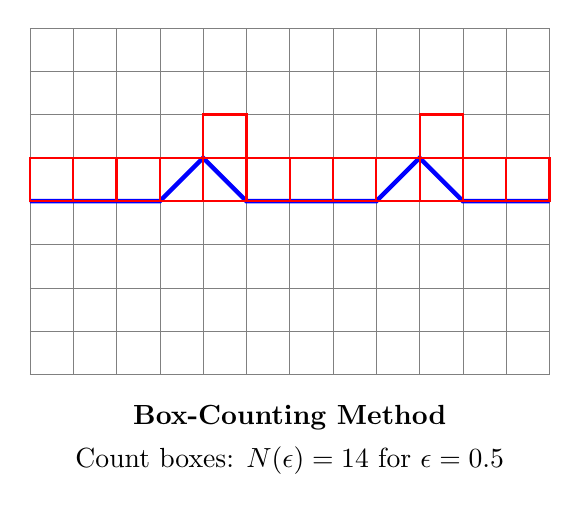
\begin{tikzpicture}[scale=1.1]
% Box-counting grid
\draw[gray, very thin, step=0.5] (0,0) grid (6,4);

% Fractal antenna (simplified Koch curve)
\draw[ultra thick, blue] (0,2) -- (1.5,2) -- (2,2.5) -- (2.5,2) -- (4,2) -- (4.5,2.5) -- (5,2) -- (6,2);

% Boxes intersecting curve
\foreach \x/\y in {0/2, 0.5/2, 1/2, 1.5/2, 2/2, 2/2.5, 2.5/2, 3/2, 3.5/2, 4/2, 4.5/2, 4.5/2.5, 5/2, 5.5/2} {
  \draw[red, thick] (\x,\y) rectangle ++(0.5,0.5);
}

\node at (3,-0.5) {\textbf{Box-Counting Method}};
\node at (3,-1) {Count boxes: $N(\epsilon) = 14$ for $\epsilon = 0.5$};
\end{tikzpicture}
\caption{Box-counting dimension measurement. Blue: fractal antenna (simplified Koch curve). Red boxes: grid cells ($\epsilon = 0.5$ units) intersecting curve. Dimension $D = \log N / \log(1/\epsilon)$.}
\label{fig:p5:box_counting}
\end{figure}

\marginnote{\textbf{Advanced}: Multi-dimensional fits combining dilepton, diphoton, and dijet channels improve sensitivity to $R < 5 \times 10^{-20}$ m.}

\section{Summary}\label{sec:p5:dim_summary}

Dimensional spectroscopy protocols span microscopic to cosmological scales:

**Quantum walks** (nm to $\mu$m): Spectral dimension extraction via return probability. Sierpinski gasket: $d_S \approx 1.58$.

**Fractal antennas** ($\mu$m to mm): Box-counting dimension from microscopy. Koch snowflake: $D_{\text{box}} \approx 1.26$.

**Laser diffraction** (mm apertures): Fourier dimension from diffraction patterns. Cantor grating: $D_F \approx 0.63$.

**Collider searches** (TeV energies): KK graviton resonances constrain extra dimension radius: $R < 10^{-19}$ m.

\marginnote{\textbf{Historical}: From Hausdorff's 1919 mathematical abstraction to 2020s experimental tests---fractional dimensions now measurable in laboratories.}

**Key Results**:
\begin{enumerate}
\item Spectral dimension quantifies diffusion efficiency on fractal geometries
\item Box-counting provides straightforward metric for self-similar structures
\item Collider null results tightly constrain large extra dimensions
\end{enumerate}

**Forward Bridges**:
\begin{itemize}
\item Paper 6 (Applications): Fractal antenna design, quantum random walk algorithms, extra-dimensional cosmology
\end{itemize}

**Concluding Remarks**:

This paper presented comprehensive experimental protocols for five exotic quantum states and fundamental physics tests:
\begin{enumerate}
\item Time crystals: Discrete time symmetry breaking, $>200$-cycle coherence
\item Quantum foam: Planck-scale probes via GRB timing, atom interferometry
\item Holographic entropy: Bekenstein-Hawking formula tests in analogue systems
\item Scalar field detection: Casimir modifications, fifth-force searches
\item Dimensional spectroscopy: Spectral dimension, Kaluza-Klein resonances
\end{enumerate}

\marginnote{\textbf{Pedagogical}: These "exotic" phenomena span from confirmed experiments (time crystals) to speculative tests (quantum foam)---representing frontier of experimental physics.}

The protocols developed here provide roadmaps for next-generation experiments pushing measurement precision toward fundamental limits set by quantum mechanics and gravity. Whether confirming Standard Model predictions or revealing new physics, these techniques advance our empirical understanding of nature's deepest structures.

\marginnote{\textbf{Cautionary}: Extraordinary claims require extraordinary evidence. All protocols emphasize rigorous error analysis, systematic mitigation, and independent replication.}

%==============================================================================
% END OF CHAPTER 5 AND PAPER 5
%==============================================================================
